\documentclass[tikz]{standalone}

%%%<
\usepackage{verbatim}
%%%>

\usepackage{fontspec}
\setsansfont{TeX Gyre Adventor}

\usepackage{tikz}
\usetikzlibrary{shapes,calc,positioning}

\begin{document}

\newcommand{\CommonElementTextFormat}[4]
{
	\begin{minipage}[t][1.5in]{1.1in}
	\textbf{\Large #1} \par
		\vfill
	\begin{center}
		\textbf{\fontsize{0.5in}{0.3in}\selectfont #3}\par
		\vfill
		{{#4}} \par
		\vfill
		{{\Large #2}}
		\vfill
	\end{center}
	\end{minipage}
}

\newcommand{\NaturalElementTextFormat}[4]
{
  \CommonElementTextFormat{#1}{#2}{#3}{#4}
}

\newcommand{\SyntheticElementTextFormat}[4]
{
  \CommonElementTextFormat{#1}{(#2)}{#3}{#4}
}

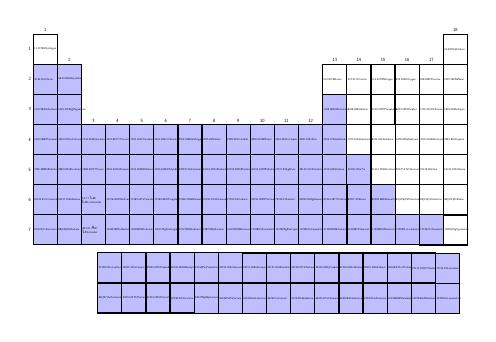
\begin{tikzpicture}[font=\sffamily, transform shape,scale=0.1]

%% Fill Color Styles
	\tikzstyle{ElementFill}            = [fill=none] %yellow!15]
	\tikzstyle{AlkaliMetalFill}        = [fill=blue!25]
	\tikzstyle{AlkalineEarthMetalFill} = [fill=blue!25]
	\tikzstyle{MetalFill}              = [fill=blue!25]
	\tikzstyle{MetalloidFill}          = [fill=none] %orange!25]
	\tikzstyle{NonmetalFill}           = [fill=none] %green!25]
	\tikzstyle{HalogenFill}            = [fill=none] %green!40]
	\tikzstyle{NobleGasFill}           = [fill=none] %green!55]
	\tikzstyle{LanthanideActinideFill} = [fill=blue!25]

%% Element Styles
  \tikzstyle{Element} = [draw=black, ElementFill,
    minimum width=1.2in, minimum height=1.5in,
	text width=1.1in, align=left]
  \tikzstyle{AlkaliMetal} = [Element, AlkaliMetalFill]
  \tikzstyle{AlkalineEarthMetal} = [Element, AlkalineEarthMetalFill]
  \tikzstyle{Metal} = [Element, MetalFill]
  \tikzstyle{Metalloid} = [Element, MetalloidFill]
  \tikzstyle{Nonmetal} = [Element, NonmetalFill]
  \tikzstyle{Halogen} = [Element, HalogenFill]
  \tikzstyle{NobleGas} = [Element, NobleGasFill]
  \tikzstyle{LanthanideActinide} = [Element, LanthanideActinideFill]
  \tikzstyle{PeriodLabel} = [font={\sffamily\LARGE}, node distance=2.0cm]
  \tikzstyle{GroupLabel} = [font={\sffamily\LARGE}, minimum width=1in, node distance=2.0cm]
  \tikzstyle{TitleLabel} = [font={\sffamily\Huge\bfseries}]

%% Group 1 - IA
  \node[name=H, Element] {\NaturalElementTextFormat{1}{1.0079}{H}{Hydrogen}};
  \node[name=Li, below =0pt of H, AlkaliMetal] {\NaturalElementTextFormat{3}{6.941}{Li}{Lithium}};
  \node[name=Na, below =0pt of Li, AlkaliMetal] {\NaturalElementTextFormat{11}{22.990}{Na}{Sodium}};
  \node[name=K,  below =0pt of Na, AlkaliMetal] {\NaturalElementTextFormat{19}{39.098}{K}{Potassium}};
  \node[name=Rb, below =0pt of K, AlkaliMetal] {\NaturalElementTextFormat{37}{85.468}{Rb}{Rubidium}};
  \node[name=Cs, below =0pt of Rb, AlkaliMetal] {\NaturalElementTextFormat{55}{132.91}{Cs}{Caesium}};
  \node[name=Fr, below =0pt of Cs, AlkaliMetal] {\NaturalElementTextFormat{87}{(223)}{Fr}{Francium}};

%% Group 2 - IIA
  \node[name=Be, right =0pt of Li, AlkalineEarthMetal] {\NaturalElementTextFormat{4}{9.0122}{Be}{Beryllium}};
  \node[name=Mg, below =0pt of Be, AlkalineEarthMetal] {\NaturalElementTextFormat{12}{24.305}{Mg}{Magnesium}};
  \node[name=Ca, below =0pt of Mg, AlkalineEarthMetal] {\NaturalElementTextFormat{20}{40.078}{Ca}{Calcium}};
  \node[name=Sr, below =0pt of Ca, AlkalineEarthMetal] {\NaturalElementTextFormat{38}{87.62}{Sr}{Strontium}};
  \node[name=Ba, below =0pt of Sr, AlkalineEarthMetal] {\NaturalElementTextFormat{56}{137.33}{Ba}{Barium}};
  \node[name=Ra, below =0pt of Ba, AlkalineEarthMetal] {\NaturalElementTextFormat{88}{(226)}{Ra}{Radium}};

%% Group 3 - IIIB
  \node[name=Sc,   right =0pt of Ca, Metal] {\NaturalElementTextFormat{21}{44.956}{Sc}{Scandium}};
  \node[name=Y,    below =0pt of Sc, Metal] {\NaturalElementTextFormat{39}{88.906}{Y}{Yttrium}};
  \node[name=LaLu, below =0pt of Y, LanthanideActinide] {\NaturalElementTextFormat{57-71}{\phantom{1}}{\vphantom{L}{\LARGE La-Lu}}{Lanthanides}};
  \node[name=AcLr, below =0pt of LaLu, LanthanideActinide] {\NaturalElementTextFormat{89-103}{\phantom{1}}{\vphantom{A}{\LARGE Ac-Lr}}{Actinides}};

%% Group 4 - IVB
  \node[name=Ti, right =0pt of Sc, Metal] {\NaturalElementTextFormat{22}{47.867}{Ti}{Titanium}};
  \node[name=Zr, below =0pt of Ti, Metal] {\NaturalElementTextFormat{40}{91.224}{Zr}{Zirconium}};
  \node[name=Hf, below =0pt of Zr, Metal] {\NaturalElementTextFormat{72}{178.49}{Hf}{Halfnium}};
  \node[name=Rf, below =0pt of Hf, Metal] {\SyntheticElementTextFormat{104}{267}{Rf}{Rutherfordium}};

%% Group 5 - VB
  \node[name=V,  right =0pt of Ti, Metal] {\NaturalElementTextFormat{23}{50.942}{V}{Vanadium}};
  \node[name=Nb, below =0pt of V, Metal] {\NaturalElementTextFormat{41}{92.906}{Nb}{Niobium}};
  \node[name=Ta, below =0pt of Nb, Metal] {\NaturalElementTextFormat{73}{180.95}{Ta}{Tantalum}};
  \node[name=Db, below =0pt of Ta, Metal] {\SyntheticElementTextFormat{105}{268}{Db}{Dubnium}};

%% Group 6 - VIB
  \node[name=Cr, right =0pt of V, Metal] {\NaturalElementTextFormat{24}{51.996}{Cr}{Chromium}};
  \node[name=Mo, below =0pt of Cr, Metal] {\NaturalElementTextFormat{42}{95.94}{Mo}{Molybdenum}};
  \node[name=W,  below =0pt of Mo, Metal] {\NaturalElementTextFormat{74}{183.84}{W}{Tungsten}};
  \node[name=Sg, below =0pt of W, Metal] {\SyntheticElementTextFormat{106}{271}{Sg}{Seaborgium}};

%% Group 7 - VIIB
  \node[name=Mn, right =0pt of Cr, Metal] {\NaturalElementTextFormat{25}{54.938}{Mn}{Manganese}};
  \node[name=Tc, below =0pt of Mn, Metal] {\NaturalElementTextFormat{43}{96}{Tc}{Technetium}};
  \node[name=Re, below =0pt of Tc, Metal] {\NaturalElementTextFormat{75}{186.21}{Re}{Rhenium}};
  \node[name=Bh, below =0pt of Re, Metal] {\SyntheticElementTextFormat{107}{272}{Bh}{Bohrium}};

%% Group 8 - VIIIB
  \node[name=Fe, right =0pt of Mn, Metal] {\NaturalElementTextFormat{26}{55.845}{Fe}{Iron}};
  \node[name=Ru, below =0pt of Fe, Metal] {\NaturalElementTextFormat{44}{101.07}{Ru}{Ruthenium}};
  \node[name=Os, below =0pt of Ru, Metal] {\NaturalElementTextFormat{76}{190.23}{Os}{Osmium}};
  \node[name=Hs, below =0pt of Os, Metal] {\SyntheticElementTextFormat{108}{270}{Hs}{Hassium}};

%% Group 9 - VIIIB
  \node[name=Co, right =0pt of Fe, Metal] {\NaturalElementTextFormat{27}{58.933}{Co}{Cobalt}};
  \node[name=Rh, below =0pt of Co, Metal] {\NaturalElementTextFormat{45}{102.91}{Rh}{Rhodium}};
  \node[name=Ir, below =0pt of Rh, Metal] {\NaturalElementTextFormat{77}{192.22}{Ir}{Iridium}};
  \node[name=Mt, below =0pt of Ir, Metal] {\SyntheticElementTextFormat{109}{276}{Mt}{Meitnerium}};

%% Group 10 - VIIIB
  \node[name=Ni, right =0pt of Co, Metal] {\NaturalElementTextFormat{28}{58.693}{Ni}{Nickel}};
  \node[name=Pd, below =0pt of Ni, Metal] {\NaturalElementTextFormat{46}{106.42}{Pd}{Palladium}};
  \node[name=Pt, below =0pt of Pd, Metal] {\NaturalElementTextFormat{78}{195.08}{Pt}{Platinum}};
  \node[name=Ds, below =0pt of Pt, Metal] {\SyntheticElementTextFormat{110}{281}{Ds}{Darmstadtium}};

%% Group 11 - IB
  \node[name=Cu, right =0pt of Ni, Metal] {\NaturalElementTextFormat{29}{63.546}{Cu}{Copper}};
  \node[name=Ag, below =0pt of Cu, Metal] {\NaturalElementTextFormat{47}{107.87}{Ag}{Silver}};
  \node[name=Au, below =0pt of Ag, Metal] {\NaturalElementTextFormat{79}{196.97}{Au}{Gold}};
  \node[name=Rg, below =0pt of Au, Metal] {\SyntheticElementTextFormat{111}{280}{Rg}{Roentgenium}};

%% Group 12 - IIB
  \node[name=Zn, right =0pt of Cu, Metal] {\NaturalElementTextFormat{30}{65.39}{Zn}{Zinc}};
  \node[name=Cd, below =0pt of Zn, Metal] {\NaturalElementTextFormat{48}{112.41}{Cd}{Cadmium}};
  \node[name=Hg, below =0pt of Cd, Metal] {\NaturalElementTextFormat{80}{200.59}{Hg}{Mercury}};
  \node[name=Cn, below =0pt of Hg, Metal] {\SyntheticElementTextFormat{112}{285}{Cn}{Copernicium}};

%% Group 13 - IIIA
  \node[name=Ga, right =0pt of Zn, Metal] {\NaturalElementTextFormat{31}{69.723}{Ga}{Gallium}};
  \node[name=Al, above =0pt of Ga, Metal] {\NaturalElementTextFormat{13}{26.982}{Al}{Aluminium}};
  \node[name=B,  above =0pt of Al, Metalloid] {\NaturalElementTextFormat{5}{10.811}{B}{Boron}};
  \node[name=In, below =0pt of Ga, Metal] {\NaturalElementTextFormat{49}{114.82}{In}{Indium}};
  \node[name=Tl, below =0pt of In, Metal] {\NaturalElementTextFormat{81}{204.38}{Tl}{Thallium}};
  \node[name=Nh, below =0pt of Tl, Metal] {\SyntheticElementTextFormat{113}{284}{Nh}{Nihonium}};

%% Group 14 - IVA
  \node[name=C,  right =0pt of B, Nonmetal] {\NaturalElementTextFormat{6}{12.011}{C}{Carbon}};
  \node[name=Si, below =0pt of C, Metalloid] {\NaturalElementTextFormat{14}{28.086}{Si}{Silicon}};
  \node[name=Ge, below =0pt of Si, Metalloid] {\NaturalElementTextFormat{32}{72.64}{Ge}{Germanium}};
  \node[name=Sn, below =0pt of Ge, Metal] {\NaturalElementTextFormat{50}{118.71}{Sn}{Tin}};
  \node[name=Pb, below =0pt of Sn, Metal] {\NaturalElementTextFormat{82}{207.2}{Pb}{Lead}};
  \node[name=Fl, below =0pt of Pb, Metal] {\SyntheticElementTextFormat{114}{289}{Fl}{Flerovium}};

%% Group 15 - VA
  \node[name=N,  right =0pt of C, Nonmetal] {\NaturalElementTextFormat{7}{14.007}{N}{Nitrogen}};
  \node[name=P,  below =0pt of N, Nonmetal] {\NaturalElementTextFormat{15}{30.974}{P}{Phosphorus}};
  \node[name=As, below =0pt of P, Metalloid] {\NaturalElementTextFormat{33}{74.922}{As}{Arsenic}};
  \node[name=Sb, below =0pt of As, Metalloid] {\NaturalElementTextFormat{51}{121.76}{Sb}{Antimony}};
  \node[name=Bi, below =0pt of Sb, Metal] {\NaturalElementTextFormat{83}{208.98}{Bi}{Bismuth}};
  \node[name=Mc, below =0pt of Bi, Metal] {\SyntheticElementTextFormat{115}{288}{Mc}{Moscovium}};

%% Group 16 - VIA
  \node[name=O,  right =0pt of N, Nonmetal] {\NaturalElementTextFormat{8}{15.999}{O}{Oxygen}};
  \node[name=S,  below =0pt of O, Nonmetal] {\NaturalElementTextFormat{16}{32.065}{S}{Sulphur}};
  \node[name=Se, below =0pt of S, Nonmetal] {\NaturalElementTextFormat{34}{78.96}{Se}{Selenium}};
  \node[name=Te, below =0pt of Se, Metalloid] {\NaturalElementTextFormat{52}{127.6}{Te}{Tellurium}};
  \node[name=Po, below =0pt of Te, Metalloid] {\NaturalElementTextFormat{84}{(209)}{Po}{Polonium}};
  \node[name=Lv, below =0pt of Po, Metal] {\SyntheticElementTextFormat{116}{293}{Lv}{Livermorium}};

%% Group 17 - VIIA
  \node[name=F,  right =0pt of O, Halogen] {\NaturalElementTextFormat{9}{18.998}{F}{Flourine}};
  \node[name=Cl, below =0pt of F, Halogen] {\NaturalElementTextFormat{17}{35.453}{Cl}{Chlorine}};
  \node[name=Br, below =0pt of Cl, Halogen] {\NaturalElementTextFormat{35}{79.904}{Br}{Bromine}};
  \node[name=I,  below =0pt of Br, Halogen] {\NaturalElementTextFormat{53}{126.9}{I}{Iodine}};
  \node[name=At, below =0pt of I, Halogen] {\NaturalElementTextFormat{85}{(210)}{At}{Astatine}};
  \node[name=Ts, below =0pt of At, Metal] {\SyntheticElementTextFormat{117}{294}{Ts}{Tennessine}}; 

%% Group 18 - VIIIA
  \node[name=Ne, right =0pt of F, NobleGas] {\NaturalElementTextFormat{10}{20.180}{Ne}{Neon}};
  \node[name=He, above =0pt of Ne, NobleGas] {\NaturalElementTextFormat{2}{4.0025}{He}{Helium}};
  \node[name=Ar, below =0pt of Ne, NobleGas] {\NaturalElementTextFormat{18}{39.948}{Ar}{Argon}};
  \node[name=Kr, below =0pt of Ar, NobleGas] {\NaturalElementTextFormat{36}{83.8}{Kr}{Krypton}};
  \node[name=Xe, below =0pt of Kr, NobleGas] {\NaturalElementTextFormat{54}{131.29}{Xe}{Xenon}};
  \node[name=Rn, below =0pt of Xe, NobleGas] {\NaturalElementTextFormat{86}{(222)}{Rn}{Radon}};
  \node[name=Og, below =0pt of Rn, Nonmetal] {\SyntheticElementTextFormat{118}{294}{Og}{Oganesson}}; 

%% Period
  \node[name=Period1, left =5pt of H, PeriodLabel] {1};
  \node[name=Period2, left =5pt of Li, PeriodLabel] {2};
  \node[name=Period3, left =5pt of Na, PeriodLabel] {3}; 
  \node[name=Period4, left =5pt of K, PeriodLabel] {4}; 
  \node[name=Period5, left =5pt of Rb, PeriodLabel] {5};
  \node[name=Period6, left =5pt of Cs, PeriodLabel] {6};
  \node[name=Period7, left =5pt of Fr, PeriodLabel] {7};

%% Group
  \node[name=Group1,  above =5pt of H, GroupLabel]   {1 }; %\hfill IA};
  \node[name=Group2,  above =5pt of Be, GroupLabel]  {2 }; %\hfill IIA};
  \node[name=Group3,  above =5pt of Sc, GroupLabel]  {3 }; %\hfill IIIA};
  \node[name=Group4,  above =5pt of Ti, GroupLabel]  {4 }; %\hfill IVB};
  \node[name=Group5,  above =5pt of V, GroupLabel]   {5 }; %\hfill VB};
  \node[name=Group6,  above =5pt of Cr, GroupLabel]  {6 }; %\hfill VIB};
  \node[name=Group7,  above =5pt of Mn, GroupLabel]  {7 }; %\hfill VIIB};
  \node[name=Group8,  above =5pt of Fe, GroupLabel]  {8 }; %\hfill VIIIB};
  \node[name=Group9,  above =5pt of Co, GroupLabel]  {9 }; %\hfill VIIIB};
  \node[name=Group10, above =5pt of Ni, GroupLabel] {10}; % \hfill VIIIB};
  \node[name=Group11, above =5pt of Cu, GroupLabel] {11}; % \hfill IB};
  \node[name=Group12, above =5pt of Zn, GroupLabel] {12}; % \hfill IIB};
  \node[name=Group13, above =5pt of B, GroupLabel]  {13}; % \hfill IIIA};
  \node[name=Group14, above =5pt of C, GroupLabel]  {14}; % \hfill IVA};
  \node[name=Group15, above =5pt of N, GroupLabel]  {15}; % \hfill VA};
  \node[name=Group16, above =5pt of O, GroupLabel]  {16}; % \hfill VIA};
  \node[name=Group17, above =5pt of F, GroupLabel]  {17}; % \hfill VIIA};
  \node[name=Group18, above =5pt of He, GroupLabel] {18}; % \hfill VIIIA};

%% Lanthanide
  \node[name=La, below =0pt of Rf, LanthanideActinide, yshift=-1cm, xshift=-1cm] {\NaturalElementTextFormat{57}{138.91}{La}{Lanthanum}};
  \node[name=Ce, right =0pt of La, LanthanideActinide] {\NaturalElementTextFormat{58}{140.12}{Ce}{Cerium}};
  \node[name=Pr, right =0pt of Ce, LanthanideActinide] {\NaturalElementTextFormat{59}{140.91}{Pr}{Praseodymium}};
  \node[name=Nd, right =0pt of Pr, LanthanideActinide] {\NaturalElementTextFormat{60}{144.24}{Nd}{Neodymium}};
  \node[name=Pm, right =0pt of Nd, LanthanideActinide] {\SyntheticElementTextFormat{61}{145}{Pm}{Promethium}};
  \node[name=Sm, right =0pt of Pm, LanthanideActinide] {\NaturalElementTextFormat{62}{150.36}{Sm}{Samarium}};
  \node[name=Eu, right =0pt of Sm, LanthanideActinide] {\NaturalElementTextFormat{63}{151.96}{Eu}{Europium}};
  \node[name=Gd, right =0pt of Eu, LanthanideActinide] {\NaturalElementTextFormat{64}{157.25}{Gd}{Gadolinium}};
  \node[name=Tb, right =0pt of Gd, LanthanideActinide] {\NaturalElementTextFormat{65}{158.93}{Tb}{Terbium}};
  \node[name=Dy, right =0pt of Tb, LanthanideActinide] {\NaturalElementTextFormat{66}{162.50}{Dy}{Dysprosium}};
  \node[name=Ho, right =0pt of Dy, LanthanideActinide] {\NaturalElementTextFormat{67}{164.93}{Ho}{Holmium}};
  \node[name=Er, right =0pt of Ho, LanthanideActinide] {\NaturalElementTextFormat{68}{167.26}{Er}{Erbium}};
  \node[name=Tm, right =0pt of Er, LanthanideActinide] {\NaturalElementTextFormat{69}{168.93}{Tm}{Thulium}};
  \node[name=Yb, right =0pt of Tm, LanthanideActinide] {\NaturalElementTextFormat{70}{173.04}{Yb}{Ytterbium}};
  \node[name=Lu, right =0pt of Yb, LanthanideActinide] {\NaturalElementTextFormat{71}{174.97}{Lu}{Lutetium}};

%% Actinide
  \node[name=Ac, below =0pt of La, LanthanideActinide,] {\NaturalElementTextFormat{89}{(227)}{Ac}{Actinium}};
  \node[name=Th, right =0pt of Ac, LanthanideActinide] {\NaturalElementTextFormat{90}{232.04}{Th}{Thorium}};
  \node[name=Pa, right =0pt of Th, LanthanideActinide] {\NaturalElementTextFormat{91}{231.04}{Pa}{Protactinium}};
  \node[name=U,  right =0pt of Pa, LanthanideActinide] {\NaturalElementTextFormat{92}{238.03}{U}{Uranium}};
  \node[name=Np, right =0pt of U, LanthanideActinide] {\SyntheticElementTextFormat{93}{237}{Np}{Neptunium}};
  \node[name=Pu, right =0pt of Np, LanthanideActinide] {\SyntheticElementTextFormat{94}{244}{Pu}{Plutonium}};
  \node[name=Am, right =0pt of Pu, LanthanideActinide] {\SyntheticElementTextFormat{95}{243}{Am}{Americium}};
  \node[name=Cm, right =0pt of Am, LanthanideActinide] {\SyntheticElementTextFormat{96}{247}{Cm}{Curium}};
  \node[name=Bk, right =0pt of Cm, LanthanideActinide] {\SyntheticElementTextFormat{97}{247}{Bk}{Berkelium}};
  \node[name=Cf, right =0pt of Bk, LanthanideActinide] {\SyntheticElementTextFormat{98}{251}{Cf}{Californium}};
  \node[name=Es, right =0pt of Cf, LanthanideActinide] {\SyntheticElementTextFormat{99}{252}{Es}{Einsteinium}};
  \node[name=Fm, right =0pt of Es, LanthanideActinide] {\SyntheticElementTextFormat{100}{257}{Fm}{Fermium}};
  \node[name=Md, right =0pt of Fm, LanthanideActinide] {\SyntheticElementTextFormat{101}{258}{Md}{Mendelevium}};
  \node[name=No, right =0pt of Md, LanthanideActinide] {\SyntheticElementTextFormat{102}{259}{No}{Nobelium}};
  \node[name=Lr, right =0pt of No, LanthanideActinide] {\SyntheticElementTextFormat{103}{262}{Lr}{Lawrencium}};

\end{tikzpicture}
\end{document}
